\afterpage{
  \centering
  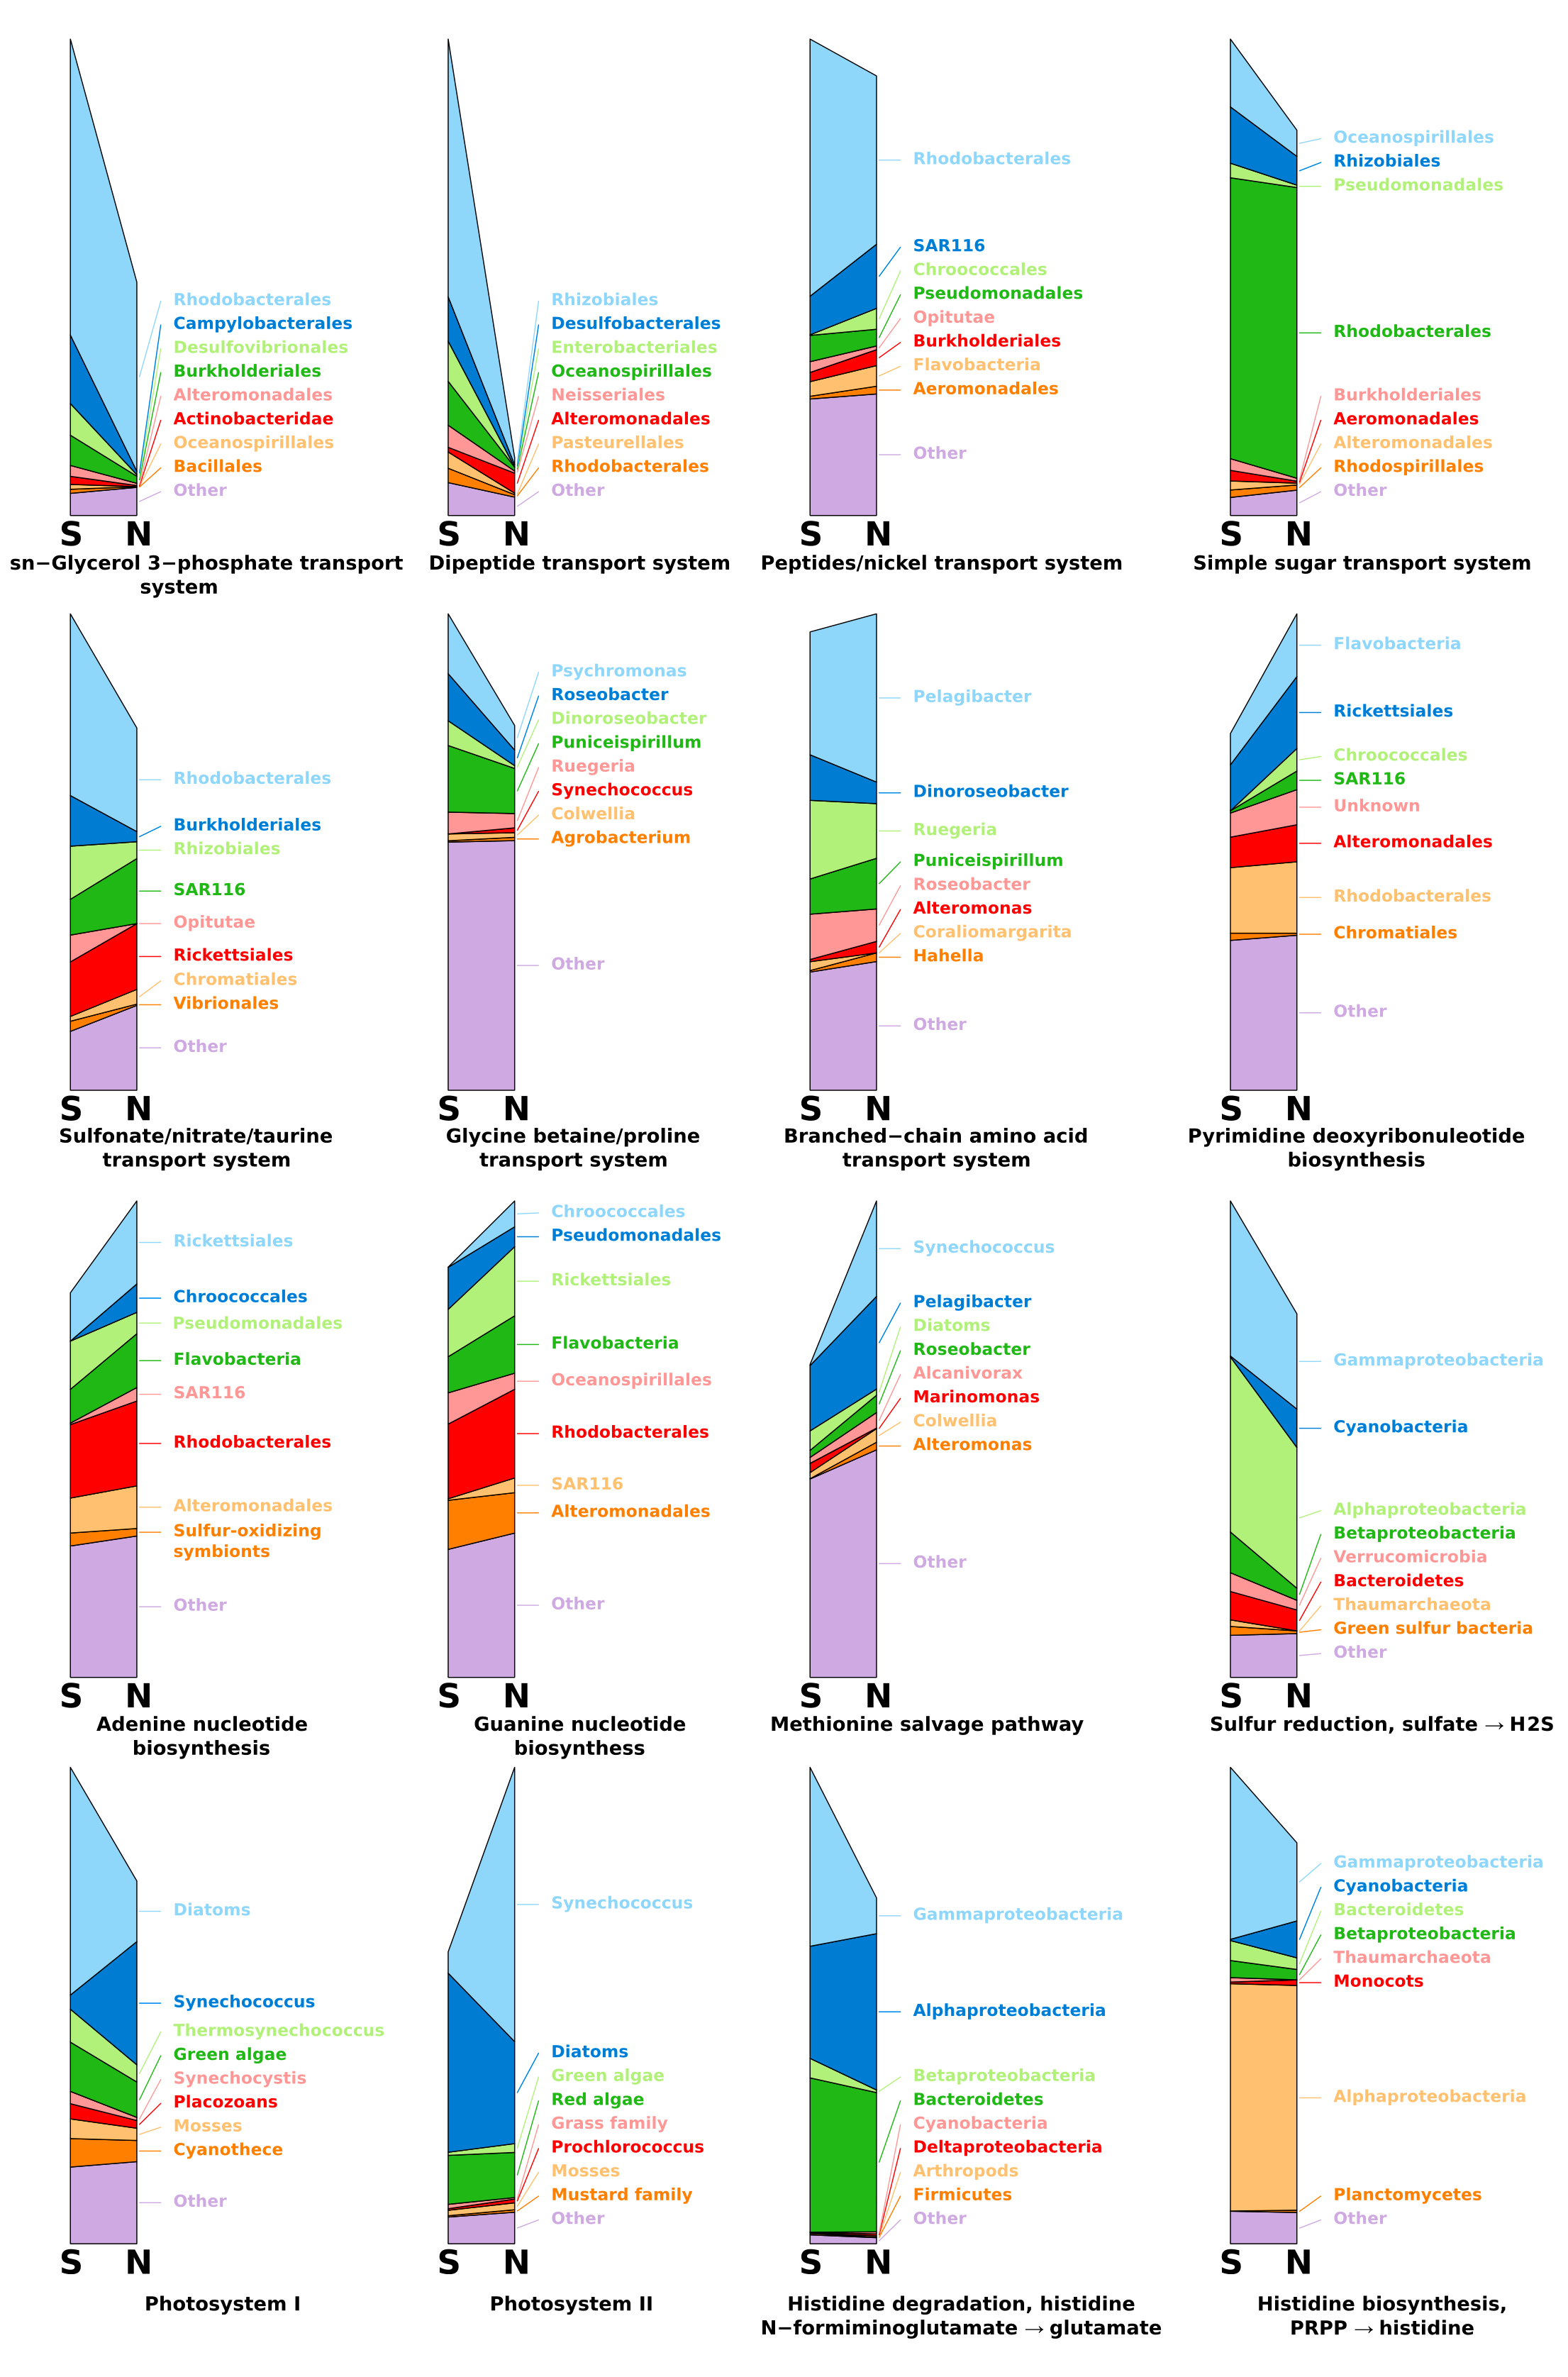
\includegraphics[width=\textwidth]{../polarfront/moduledecomp.png}
  \captionof{figure}[Taxonomic decomposition of KEGG modules]{\sffamily{}Decomposition of KEGG modules of interest to contributing classes, orders or genera. The left side of each stack (S) indicates the proportion of the module abundance contributed by each class, order or genus in the South Zone, while the right side (N) represents the North Zone. As the contributions are relative and represent unitless module abundances, no axis is given and proportions are not comparable between modules. Contributing classes, orders or genera are arranged in descending order of the difference in the relative contributions between the zones. Only the eight highest contributors for each module are shown, with the remainder collapsed into the ``Other'' group. The taxonomic ranks to which each module was decomposed are as follows: sn-glycerol 3-phosphate transport, peptide-nickel transport, simple sugar transport and sulfonate/nitrate/taurine transport were decomposed to order; glycine betaine/proline transport and branched-chain amino acid transport to genus; pyrimidine deoxyribonucleotide biosynthesis, adenine nucleotide biosynthesis and guanine nucleotide biosynthesis to order; methionine salvage to genus; sulphur reduction to class; photosystem I and photosystem II to genus; histidine degradation to glutamate and histidine biosynthesis to class.\\
  \rule[1ex]{2cm}{0.5pt}
  }
  \label{fig:moduledecomp}
}
